\documentclass[12pt,a4paper,final]{article}
\usepackage[utf8]{inputenc}
\usepackage[russian]{babel}
\usepackage[OT1]{fontenc}
\usepackage{amsmath}
\usepackage{amsfonts}
\usepackage{amssymb}
\usepackage{hyperref}
\usepackage{graphicx}
\usepackage{xcolor}
\usepackage{tikz}
\usepackage{todonotes}

\usetikzlibrary{arrows,matrix,positioning}

\DeclareMathOperator{\T}{T}
\DeclareMathOperator{\tr}{tr}
\DeclareMathOperator{\Tr}{Tr} 
\DeclareMathOperator{\MSE}{MSE} 
\DeclareMathOperator{\E}{E}
\DeclareMathOperator{\D}{D}

\DeclareMathOperator{\rank}{rank}
\DeclareMathOperator{\diam}{diam}
\DeclareMathOperator{\ob}{Ob}
\DeclareMathOperator{\Hom}{Hom}
\DeclareMathOperator{\sign}{sign}
\DeclareMathOperator{\var}{Var}
\DeclareMathOperator{\bias}{Bias}
\newcommand{\sgn}{\text{sgn}}
\newcommand{\betah}{\hat{\bm \beta}}
\newcommand{\betaa}{\bm{\beta}}
\newcommand{\epss}{\bm{\varepsilon}}
%\newcommand{\E}{\mathrm{E}}
%\newcommand{\D}{\mathrm{D}}
\newcommand{\XT}{{\bm{X}}^{\mathrm{T}}}
\newcommand{\X}{\bm{X}}
\newcommand{\y}{\bm{y}}
\newcommand{\1}{\mathds{1}}
\newcommand{\prob}{\mathrm{P}}
\DeclareMathOperator*{\argmax}{arg\,max}
\DeclareMathOperator*{\argmin}{arg\,min}
\newtheorem{definition}{Определение}
\newtheorem{theorem}{Теорема}
\usepackage{bm}
\usepackage[left=2cm,right=2cm,top=2cm,bottom=2cm]{geometry}

\newtheorem{proposition}{Предложение}

\author{Михаил Козак, Павел Мехнин, Данил Шкурат}
\title{Регрессия, регуляризация, отбор признаков}
\begin{document}
\maketitle
%\tableofcontents

\newpage

\section{Обучение с учителем}

Обучение с учителем — это направление машинного обучения, объединяющее алгоритмы и методы построения моделей на основе множества примеров, содержащих пары «известный вход — известный выход». Иными словами, чтобы алгоритм относился к обучению с учителем, он должен работать с примерами, которые содержат не только вектор независимых переменных (атрибутов, признаков), но и значение, которое должна выдавать модель после обучения (такое значение называется целевым). Разность между целевым и фактическим выходами модели называется ошибкой обучения (невязкой, остатками), которая минимизируется в процессе обучения.


\section{Регрессия}

Рассмотрим задачу обучения с учителем, частным случаем которой является задача регрессии.

$\bf X$ --- множество объектов, заданное своими признаками (точки $p$-мерного пространства)
	
$\bf Y$ --- множество ответов (действительные числа) 
	
Предполагаем наличие неизвестной зависимости между объектами $\mathbf x \in \bf X$ и ответами $y \in \bf Y$: $$y = f^*(\mathbf x) + \epss$$
	
$(\mathbf x_i,y_{i})_{i=1}^{n}$ --- обучающая выборка (пары объект-известный ответ), случайным образом выбранная из генеральной совокупности.
\\
\\	
\textbf{Задача}:

На основе обучающей выборки найти $\hat f$, такую что $y \approx 
\hat f(\mathbf x)$ для любого наблюдения $(\mathbf x, y)$, то есть восстановить зависимость, способную для любого объекта выдать достаточно точный ответ.

Для того, чтобы данная задача была корректной, нужно, чтобы все рассматриваемые объекты были в некотором смысле однородны и происходили из некоторой генеральной совокупности (если иначе, то как предсказать ответ, когда новый объект $\mathbf x_i$ совершенно не похож на объекты обучающей выборки).

В машинном обучении для обоснования использования методов регрессии используется так называемая гипотеза непрерывности: <<близким>> объектам $\mathbf x_i$ соответствуют <<близкие>> ответы $y_i$.

\subsection{Задача регрессии как задача оптимизации}

Пусть дана обучающая выборка $X_{n}=(\mathbf x_i,y_{i})_{i=1}^{n}$, где $\mathbf x_i\in\mathbb{R}^{p}$, $y_{i}\in\mathbb{R}$ и предполагается, что между ответами и объектами есть связь:
\begin{equation*}
	y_{i}=f^{\ast}(\mathbf x_i)+\varepsilon_{i},
	\qquad 
	i=1,\ldots,n.
\end{equation*}
где $\varepsilon_{i}$ --- независимые одинаково распределенные случайные величины с $\mathbb{E}\varepsilon_{i}=0$, $\mathbb{E}\varepsilon_{i}^{2}=\sigma^{2}$.

Пусть задана модель регрессии --- параметрическое семейство функций $f(\mathbf x,\bm\beta)$, где $\bm\beta\in \bm B$ --- вектор параметров модели, $\bm B\subset\mathbb{R}^{p}$ --- пространство параметров,
$f:\mathbb{R}^{p}\times \bm B\rightarrow\mathbb{R}$ --- фиксированная функция.

Выберем в качестве функционала качества $Q$ аппроксимации целевой зависимости на выборке $X_{n}$ среднеквадратическую ошибку:
\begin{equation}\label{eq:MSE}
	\MSE_{\text{train}}
	=
	Q(\bm\beta,X_{n})=
	\frac{1}{n}
	\sum_{i=1}^{n}
	(f(\mathbf x_{i},\bm\beta)-y_{i})^{2}.
\end{equation}

Обучение по методу наименьших квадратов (МНК) состоит в нахождении такого вектора параметров $\hat{\bm\beta}$, при котором достигается минимум среднего квадрата ошибки на заданной обучающей выборке $X_{n}$:
\begin{equation*}
	\hat{\bm\beta}=
	\arg\min_{\bm\beta \in\mathbb{R}^{p}}
	Q(\bm\beta,X_{n}).
\end{equation*}

$\MSE$ в \eqref{eq:MSE} вычисляется на основе обучающей выборки, то есть наблюдений, которые были использованы для подгонки модели, так что это ошибка на обучающей выборке. В реальности нас интересует ошибка $\MSE$ на контрольной выборке, то есть то, насколько метод дает точное предсказание для наблюдений, которые не участвовали в оценке $f^{\ast}$. 
Нет гарантии, что метод с минимальной среднеквадратической ошибкой на обучающих данных также будет иметь минимальную $\MSE$ на контрольных данных.

Когда качество работы алгоритма на новых объектах, не вошедших в состав обучения, оказывается существенно хуже, чем на обучающей выборке ($\mathrm{MSE_{\text{test}}}\gg\mathrm{MSE}_{\text{train}}$), говорят об эффекте переобучения (overtraining) или переподгонки (overfitting).


\section{Линейная регрессия}

Частным случаем задачи регрессии является линейная регрессия. Мы делаем предположение о том, что модель данных имеет следующий вид:
\begin{equation}
	\bm y = \X \betaa + \epss,
\end{equation}
где 
\begin{itemize}
	\item $\bm y \in \mathbb R^n$ --- вектор ответов,  $\epss \in \mathbb R^n$ --- вектор ошибок;
	\item $\X \in \mathbb R^{n \times p}$ --- матрица данных (детерминированная --- для простоты предполагаем, что случайность в модели происходит только от вектора шума);

	\item $\betaa \in \mathbb R^p$ --- вектор параметров;
	\item $n\geqslant p.$
\end{itemize}

Заметим, что такое предположение обосновано не только простотой результирующей модели. Если столбцы матрицы $\X$ (то есть признаки) и вектор $\y$ распределены нормально, то известно, что $\y$ является \textit{линейной} 	комбинацией столбцов матрицы $\X$.


На случайную ошибку обычно накладываются следующие требования:
\begin{equation}
	\mathbb{E}\varepsilon_i = 0,\, \mathbb{E} \varepsilon_i^2 = \sigma^2 < +\infty,\,  \mathbb{E} \varepsilon_i \varepsilon_j = 0.
	\label{req:err}
\end{equation}
Решение задачи линейной регрессии --- вектор $\betah$. 

Если не оговорено иное, под задачей линейной регрессии подразумевается задача минимизации квадратичной функции потерь:

Задача оптимизации (с квадратичной функцией потерь):

$$\betah = \argmin_{\betaa}{\|\bm y - \bm X \betaa\|^2_2}.$$

Полученную оценку $\betah_{\text{МНК}}$ называют оценкой по методу наименьших квадратов (МНК-оценкой). Она имеет явный вид (если матрица $\XT \X$ невырожденная):\footnote{берутся частные производные по компонентам вектора $\betaa$ функции потерь и приравниваются к нулю. В результате получаем уравнение, которое и даёт указанную оценку.}
\begin{equation}
	\betah_{\text{МНК}} = (\XT \X)^{-1}\XT \y.
	\label{eq:lse}
\end{equation}

Математическое ожидание полученной оценки:
\begin{multline}
	\mathbb{E} \betah_{\text{МНК}} = \E [(\XT \X)^{-1}\XT \y] = (\XT \X)^{-1}\XT \E \y = (\XT \X)^{-1}\XT \E (\X \betaa + \epss) = \\ = (\XT \X)^{-1}\XT \E (\X \betaa) + (\XT \X)^{-1}\XT \underbrace{\E \epss}_{= 0}) = (\XT \X)^{-1}\XT \E (\X \betaa) = \\ = \underbrace{(\XT \X)^{-1}(\XT\X)}_{= \mathbf I}\betaa = \betaa
\end{multline}
Таким образом, оценка $\betah_{\text{МНК}}$ является \textit{несмещённой}. 

Ковариационная матрица полученной оценки:
\begin{equation}
	\mathrm{Cov}{\betah_{\text{МНК}}} = \sigma^2 (\XT\X)^{-1}.
	\label{eq:var}
\end{equation}

Теорема Гаусса–Маркова утверждает, что $\betah_{\text{МНК}}$ имеет
наименьшую дисперсию среди всех несмещённых оценок (best
linear unbiased estimate — BLUE).

Наличие явного вида решения крайне удобно в вычислительном плане. 
Оценка вычисляется достаточно быстро посредством применения сингулярного разложения матрицы данных $\X$.


\subsection{Вычисление МНК-оценки: сингулярное разложение}

\textit{Сингулярным разложением} матрицы $\X$ называется разложение $\X = \bm V \bm D \bm U^\mathrm T$, где
\begin{itemize}
\item $\bm V$ и $\bm U$ --- ортогональные,\footnote{основное свойство ортогональных матриц: $\bm V^\mathrm T =\bm V^{-1}$ (используется при выводе формулы для $\betah_{\text{МНК}}$)} $\bm D$ --- диагональная;
\item $\bm V = (V_1, V_2, \ldots, V_n) \in \mathbb R^{n\times n}$, $V_i$ --- собственные векторы $\X \XT$;
\item $\bm U = (U_1, U_2, \ldots, U_n) \in \mathbb R^{p\times n}$, $U_i$ --- собственные векторы $\XT \X$;
\item $\bm D = \mathrm{diag}(\sqrt{\lambda_1}, \ldots,\sqrt{\lambda_n})$, $\lambda_j \geqslant 0$ --- собственные значения $\XT \X$.
\end{itemize}
Для простоты предположим, что имеем дело с матрицей полного ранга, $p = n$ (результаты распространяются на случай $n>p$).

Подставим в формулу для $\betah_{\text{МНК}}$ вместо матрицы $\X$ её сингулярное разложение и получим
\begin{multline}
  \label{eq:sing}
  \betah_{\text{МНК}} =\\= (\XT \X)^{-1}\XT \y = (\bm U \bm D \bm V^\mathrm T \bm V \bm D \bm U^\mathrm T)^{-1} \bm U \bm D \bm V^\mathrm T \y = (\bm U \bm D \bm V^{-1} \bm V \bm D \bm U^\mathrm T)^{-1} \bm U \bm D \bm V^\mathrm T \y = \\
  = (\bm U \bm D^2 \bm U^\mathrm T)^{-1} \bm U \bm D \bm V^\mathrm T \y = \bm U \bm D^{-2} \bm U^\mathrm T \bm U \bm D \bm V^\mathrm T \y =\\= \bm U \bm D^{-1} \bm V^\mathrm T \y,
\end{multline}
где $\bm D^{-1} = \mathrm{diag} (1/\sqrt{\lambda_1}, \ldots, 1/\sqrt{\lambda_n})$.

\begin{equation}
	\betah_{\text{МНК}}
	=
	\sum_{j=1}^{p}
	\frac{1}{\sqrt{\lambda_{j}}}
	U_{j}(V_{j}^{\mathrm{T}} \bm y)
\end{equation}

Если предположить, что вычисление сингулярного разложения на компьютере происходит быстро и с малой погрешностью (в целом так и есть), то такой подход к вычислению $\betah_{\text{МНК}}$ оказывается наиболее предпочтительным.

\subsection{Мультиколлинеарность}

Проблема мультиколлинеарности является общей для многих методов корреляционного анализа. МНК не исключение. 

Если матрица данных содержит несколько сильно коррелированных признаков, то есть матрица начинает приближаться к вырожденной, то минимальное собственное число становится близким к $0$.
Что будет происходить в таком случае с МНК-оценкой? 

При очень малых собственных числах $\lambda_{j}$ соответствующие знаменатели в формулах вычисления $\betah_{\text{МНК}}$ близки к нулю. Поэтому в суммах появляются очень большие и неустойчивые слагаемые.

Теряется интерпретируемость оценок коэффициентов, так как коэффициенты могут неоправданно принимать очень большие значения. 

Высокая дисперсия $\betah_{\text{МНК}}$ приводит к высокой MSE.

Ответы на контрольной выборке неустойчивы (переобучение).
\\
\\
\textbf{Способы решения проблемы:}
\begin{itemize}
	\item Регуляризация: проблема зарождается в мультиколлинеарности, а проявляется в том, что норма вектора коэффициентов увеличивается. Регуляризация контролирует увеличение нормы вектора.
	\item Преобразование признаков (feature extraction, feature engineering). Ещё одно решение проблемы мультиколлинеарности заключается в том, чтобы подвергнуть исходные признаки некоторому функциональному преобразованию, гарантировав линейную независимость новых признаков, и, возможно, сократив их	количество, то есть уменьшив размерность задачи. В методе главных компонент (principal component analysis, PCA) строится минимальное число новых признаков, по которым исходные признаки восстанавливаются линейным преобразованием с минимальными погрешностями.
	\item Отбор признаков (feature selection).
\end{itemize}



\section{Регуляризация}

Хорошая оценка $\betah$ должна иметь низкую среднеквадратическую ошибку 
\begin{equation*}
	\label{eq:mse}
	\mathbb{E}(\betaa - \betah)^2 = \underbrace{\mathbb D \betah}_{\text{дисперсия}} + \underbrace{(\mathbb E \betah - \betaa)^2}_{\text{смещение}}.
\end{equation*}

Несмещенная МНК-оценка не гарантирует минимизацию всей $\mathrm{MSE}$.
Когда матрица $\bm{X}$ близка к вырожденной (это может произойти из-за наличия мультиколлинеарности или когда число предикторов $p$ почти равно числу наблюдений $n$), дисперсия $\hat{\bm \beta}$ становится большой и $\mathrm{MSE}_{\mathrm{test}}$ увеличивается.  При $p>n$ или при полностью коллинеарных признаках оценки по методу наименьших квадратов не имеют уникального решения.

Введение небольшого смещения в оценке может привести к значительному уменьшению дисперсии и тем самым уменьшению $\mathrm{MSE}_{\text{test}}$.

\subsection{Гребневая регрессия (Ridge regression)}


\subsubsection{Задача гребневой регрессии}
Вводится штраф за увеличение нормы вектора $\bm \beta$ и минимизируется следующая функция:
\begin{equation*}
	Q_{\tau}(\bm \beta)
	=
	||\bm{X} \bm \beta-\bm y||^{2}
	+
	\tau||\bm \beta||^{2}
	\rightarrow\min_{\bm \beta},
\end{equation*}
где $\tau$ --- неотрицательный параметр регуляризации.

В развернутом виде задача оптимизации записывается так:
\begin{equation*}
	\sum_{i=1}^{n}
	\left(
	y_{i}
	-
	\sum_{j=1}^{p}\beta_{j}x_{ij}
	\right)^{2}
	+
	\tau\sum_{j=1}^{p}\beta_{j}^{2}
	\rightarrow\min_{\bm \beta}.
\end{equation*}

Решение задачи гребневой регрессии:
\begin{equation*}
	\hat{\bm \beta}_{\text{ridge}}
	=
	(\bm{X}^{\mathrm{T}}\bm{X}+\tau\bm{I}_{p})^{-1}\bm{X}^{\mathrm{T}} \bm y.
\end{equation*}



Подход на основе сингулярного разложения позволяет подбирать параметр $\tau$, вычислив SVD только один раз.

Решение гребневой регрессии через SVD:
\begin{equation*}
	\hat{\bm \beta}_{\text{ridge}}
	= \sum_{j=1}^p \frac{\sqrt{\lambda_j}}{\lambda_j + \tau} U_j(V_j^{\T}Y).
\end{equation*}


\subsubsection{Параметр регуляризации}
Чем больше коэффициент регуляризации $\tau$, тем устойчивее решение, но больше смещение. 
Когда $\tau = 0$, гребневая регрессия совпадает с обычной регрессией, но при $\tau \rightarrow \infty$ коэффициенты регрессии стремятся к нулю.
Для каждого значения $\tau$ гребневая регрессия порождает свой оптимальный набор оценок коэффициентов $\hat\beta_{1},\ldots,\hat\beta$.
Важно подобрать хорошее значение параметра $\tau$, чтобы достичь компромисса между смещением и неустойчивостью. 

Таким образом, необходимо один раз произвести сингулярное разложение матрицы $\bm {X}$, а затем несложным образом вычислять вектор оценок параметров для интересующих значений параметра $\tau$. 

Добавление в знаменатель положительного числа $\tau$ приводит к тому, что проблема неустойчивости уходит. 

\subsubsection{Подбор параметра $\tau$}
	\textbf{Скользящий контроль}:
\begin{itemize}
	\item выбираем сетку значений $\tau$;
	\item вычисляем ошибку кросс-проверки для каждого значения $\tau$;
	\item выбираем $\tau$ с наименьшим значением ошибки кросс-проверки;
	\item перестраиваем модель со всеми наблюдениями с выбранным значением $\tau$.
\end{itemize}

\textbf{Эвристика }

Скользящий контроль --- вычислительно трудоёмкая процедура. Известна практическая рекомендация брать брать $\tau$ в отрезке $[0.1, 0.4]$, если столбцы матрицы $\bm{X}$ заранее стандартизованы.

\subsubsection{Проблемы и замечания}
\begin{itemize}
	\item Стандартные МНК-оценки инварианты относительно умножения признака на константу, то есть значение $X_{j}\hat{\beta_j}$ не зависит от масштаба $j$-го признака. Оценки МНК гребневой регрессии не обладают свойством инвариантности и могут существенно меняться.	Поэтому гребневую регрессию нужно использовать после стандартизации признаков.
	\item  В конечную модель входят все начальные признаки, если признаков много, то усложняется интерпретация.
\end{itemize}


\subsection{Лассо (Lasso)}

С задачей отбора признаков справляется Лассо регрессия, в которой в качестве штрафа на норму коэффициентов используется $l_{1}$-норма вектора коэффициентов.


\subsubsection{Задача Lasso-регрессии}

Метод LASSO решает следующую задачу минимизации:
\begin{equation*}
	||\bm{X} \bm \beta - \bm y||_{2}^{2}
	+
	\tau||\bm \beta||_{1}
	\rightarrow\min_{\bm \beta},
\end{equation*}
где $\tau$ --- неотрицательный параметр регуляризации.

Задача оптимизации в развернутом виде:
\begin{equation*}
	\sum_{i=1}^{n}
	\left(
	y_{i}
	-
	\sum_{j=1}^{p}\beta_{j}x_{ij}
	\right)^{2}
	+
	\tau\sum_{j=1}^{p}|\beta_{j}|
	\rightarrow\min_{\beta_{1},\ldots,\beta_{p}}.
\end{equation*}

Сложность задачи состоит в ее негладкости, из-за которой мы не можем сразу применить теорему Куна-Таккера.

Задачу lasso-оптимизации можно переписать в форме с ограничениями: %(метод множителей Лагранжа)
\begin{equation*}
	\begin{cases}
		\sum_{i=1}^{n}
		\left(
		y_{i}
		-
		\sum_{j=1}^{p}\beta_{j}x_{ij}
		\right)^{2}
		\to
		\min_{\beta_{1},\ldots,\beta_{p}},\\
		\sum_{j=1}^{p}|\beta_{j}|\leq\ae,
	\end{cases}
\end{equation*}
где $\ae=1/\tau$.

Приведем задачу к каноничному виду. Представим каждый параметр $\beta_{j}$ в виде разности положительной и отрицательной частей: $\beta_{j}=\beta_{j}^{+}-\beta_{j}^{-}$. Тогда $|\beta_{j}|=\beta_{j}^{+}+\beta_{j}^{-}$. После замены переменных переходим к задаче 
($2p$ переменных, $2p+1$ ограничений):
\begin{equation*}
	\begin{cases}
		\sum_{i=1}^{n}
		\left(
		y_{i}
		-
		\sum_{j=1}^{p}(\beta_{j}^{+}-\beta_{j}^{-})x_{ij}
		\right)^{2}
		\to
		\min_{\beta_{1}^{+},\ldots,\beta_{p}^{+},\beta_{1}^{-},\ldots,\beta_{p}^{-}},\\
		\sum_{j=1}^{p}\beta_{j}^{+}+\beta_{j}^{-}\leq\ae,
		\quad
		\beta_{j}^{+}\geq 0,
		\quad
		\beta_{j}^{-}\geq 0.
	\end{cases}
\end{equation*}

Получили выпуклую задачу квадратичного программирования с линейными ограничениями-неравенствами, к которой применима теорема Куна-Таккера.

Чем меньше параметр $\ae$, тем больше ограничений обращаются в равенства: $\beta_{j}^{+}=\beta_{j}^{-}=0$, что соответствует обнулению коэффициента $\beta_{j}$ и исключению $j$-го признака.


\subsection{Сравнение гребневой регрессии и Лассо}

Сначала заметим, что задачу гребневой регрессии можно  представить в виде задачи минимизации с ограничениями
\begin{equation*}
	\begin{cases}
		\sum_{i=1}^{n}
		\left(
		y_{i}
		-
		\sum_{j=1}^{p}\beta_{j}x_{ij}
		\right)^{2}
		\to
		\min_{\beta_{1},\ldots,\beta_{p}},\\
		\sum_{j=1}^{p}\beta_{j}^{2}\leq\ae.
	\end{cases}
\end{equation*}


Ранее мы также получали соответствующую форму записи для лассо-регрессии:
\begin{equation*}
	\begin{cases}
		\sum_{i=1}^{n}
		\left(
		y_{i}
		-
		\sum_{j=1}^{p}\beta_{j}x_{ij}
		\right)^{2}
		\to
		\min_{\beta_{1},\ldots,\beta_{p}},\\
		\sum_{j=1}^{p}|\beta_{j}|\leq\ae.
	\end{cases}
\end{equation*}

Рассмотрим простой случай, когда $p = 2$. Тогда выражение $\sum_{i=1}^n(y_i - \sum_{j=1}^p \beta_j x_{ij})^2$ --- это эллипс с центром в точке $\hat{\bm\beta}$. Предположим, что центр эллипса не удовлетворяет ограничениям $\sum_{j = 1}^p \beta_j^2 \leq\ae$ и $\sum_{j = 1}^p |\beta_j| \leq \ae$, то есть лежит вне круга в случае гребневой регрессии и вне ромба в случае Лассо. Тогда решения задач минимизации будут лежать на границе возможных значений. 
\begin{figure}[h]
	\center{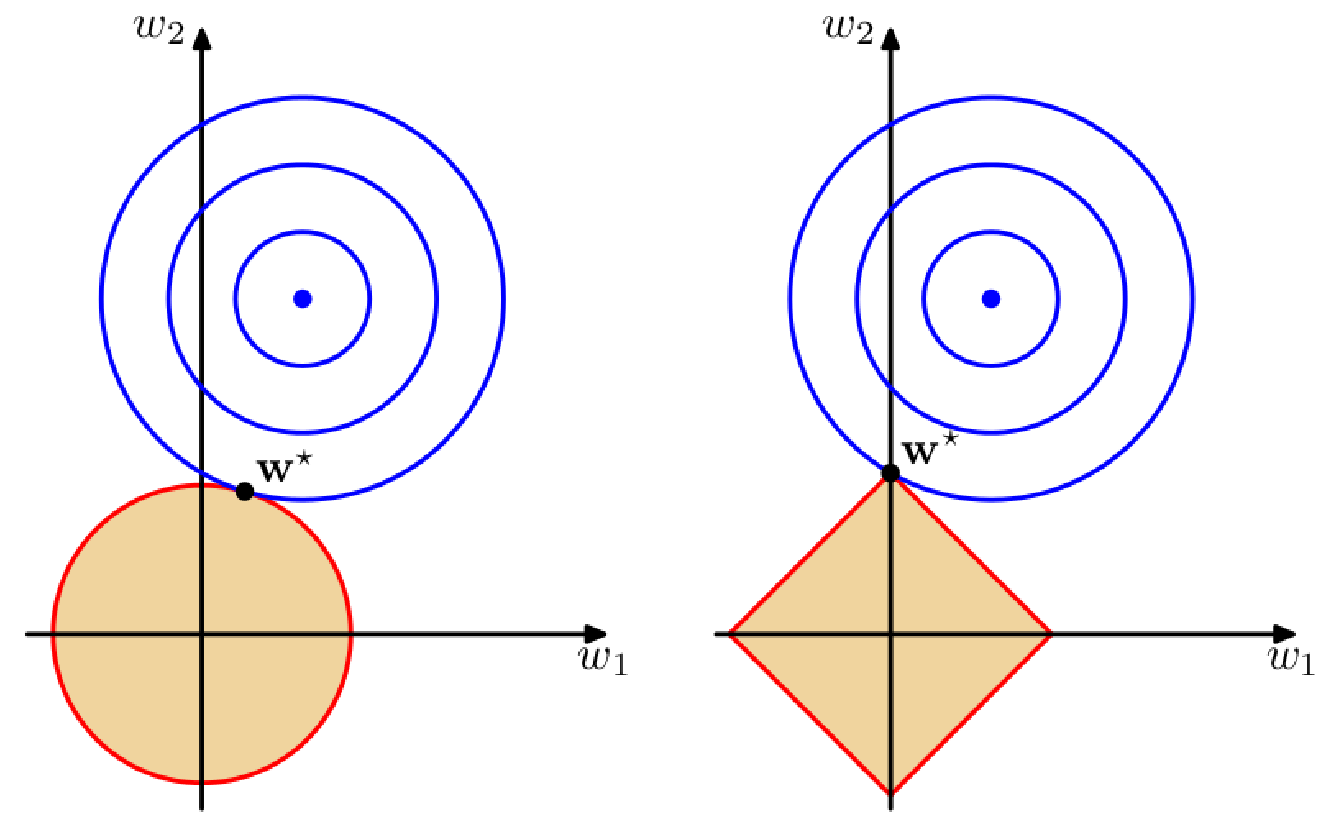
\includegraphics[width=1\linewidth]{reg.jpg}}
	\caption{Синие линии уровня функционала качества (синяя точка --- безусловный минимум, который достигается на МНК решении). Оранжевая зона --- ограничения, задаваемые L2 и L1-регуляризаторами. Чёрная точка --- минимум целевой функции при заданном ограничении.}
\end{figure}



\textbf{Замечания:}
\begin{itemize}
	\item Оба метода успешно решают проблему мультиколлинеарности
\item Гребневая регрессия использует все признаки
\item Лассо производит отбор признаков, что предпочтительнее, если среди признаков есть шумовые или измерения признаков связаны с ощутимыми затратами.
\item С помощью кросс-валидации можно определить какой подход лучше для конкретных данных.
\end{itemize}

\subsection{Elastic net regularization}
Решается задача оптимизации
\begin{equation*}
	||\bm y -\bm{X} \bm \beta||_{2}^{2} + \tau_{1}||\bm \beta ||_{1}+\tau_{2}||\bm \beta||_{2}^{2}
	\rightarrow\min_{\bm \beta}.
\end{equation*}
\begin{itemize}
	\item Elastic net --- это комбинация методов Lasso и Ridge:
	\begin{itemize}
		\item когда $\tau_1 = 0$: Ridge регрессия;
		\item когда $\tau_2 = 0$: Lasso регрессия;
	\end{itemize}
	\item Elastic net обычно дает лучшие результаты (регрессионная модель обладает лучшей предсказательной способностью), чем Lasso, при наличии коррелированных признаков;
	\item При наличии группы релевантных и избыточных признаков Lasso обычно имеет тенденцию отказываться от всех, кроме одного признака из этой группы, в то время как Elastic net будет выбирать всю группу признаков.
	\item  Если количество признаков $p$ больше, чем количество наблюдений $n$, Lasso выберет не более $n$ ненулевых предикторов (даже если все $p$ предикторов актуальны), поэтому в случае многомерных данных с малым числом наблюдений предпочтительней использовать Elstic net.
	\item Elastic net можно свести к SVM, для которого разработано много быстрых решений.
	
\end{itemize}


\section{Отбор признаков}
 
Меньшее число признаков улучшает интерпретируемость модели и уменьшает время обучения, поэтому целесообразно выбрать модель, имеющую хорошую предсказательную способность при относительно небольшом числе признаков. 
Модели обычно сравниваются с помощью информационных критериев AIC, BIC (представляют из себя функцию правдоподобия выборки с поправкой-штрафом, зависящей от числа параметров), скорректированного коэффициента детерминации $\text{adj.}R^2$ (доля объясненной дисперсии с некоторым штрафом за размерность пространства параметров).

В результате применения метода lasso получается вектор коэффициентов с большим количеством нулей, что приводит к итоговой модели с малым числом признаков. По сути, осуществляется процедура \textit{отбора признаков}.  
Рассмотрим ещё несколько подходов к решению задачи отбора признаков: best subset selection, а также forward- и backward- subset selection.

\paragraph{Best subset selection}

Если имеется $p$ признаков, наивный вариант --- рассмотреть все возможные модели с $\tilde p = 1$ признаком, $\tilde p = 2$, и так далее до $\tilde p = p$, а затем выбрать наилучшую. Количество таких моделей будет равно $2^p$. Если для примера взять $p = 20$, получим, что $2^p = 1,048,576$. Это уже довольно большое число моделей. При $p > 40$ данный подход становится затруднительным даже для построения МНК-оценок.

Также заметим, что из-за рассмотрения большого числа моделей, применение метода best subset selection может привести к проблеме переобучения (происходит подгонка модели под тренировочную выборку).

\paragraph{Forward и backward subset selection}

Также существуют и <<жадные>> альтернативы методу best subset selection. Один из вариантов (\textit{Forward subset selection}) состоит в выборе наилучшей модели с одним признаком, а затем последовательное добавление признаков, которые оказывают наилучшее влияние на критерий выбора. В итоге получаем $p(p+1)/2$ моделей. Например, для $p = 20$ получаем $210$ моделей --- значительно меньше, чем у best subset. Далее можем выбирать на основании желаемого числа признаков или опять же на основании тех же критериев. 

Аналогично можно начинать со всех признаков и последовательно удалять по одному, пока не придём к модели с одним признаком (\textit{Backward subset selection}). В случае, когда $p>n$ и считаются МНК-оценки (к примеру), метод Backward subset selection уже не сработает, так как нет возможности начать процедуру с полного пространства признаков.

\section{Источники и рекомендуемая литература}

\begin{itemize}
	\item ESL (Elements of Statistical Learning) --- Hastie, Tibshirani, Friedman;
	\item ISLR (An Introduction to Statistical Learning) --- James, Witten, Hastie, Tibshirani;
	\item Лекции Н.Э. и А.И., СтатМод;
	\item Лекции Воронцова по ML;
	\item Лекции Соколова (ФКН ВШЭ);	
	\item Лекции Larry Wasserman --- Statistical Learning;
	\item All of Statistics --- Larry Wasserman.
	
	\item https://ml-handbook.ru/

	\end{itemize}

\end{document}


